\documentclass[letter]{article}
\renewcommand{\baselinestretch}{1.25}

\usepackage[margin=1in]{geometry}
\usepackage{physics}
\usepackage{amsmath}
\usepackage{graphicx}
%\usepackage[language=Python]{listings}
\usepackage{pythonhighlight}


\newcommand{\CPS}{cyber-physical system}
\newcommand{\DT}{discrete-time}

\allowdisplaybreaks

%opening
\title{MECH 6327 - Homework 1}
\author{Jonas Wagner}
\date{2021, February 3}

\begin{document}

\maketitle

\section{Optimization Problem Formulation}
Find and research an example (ideally from your own research experience/interests) of an optimization problem in the real world. Write a short narrative of around 300 words to describe the
optimization variables, objective function(s), constraint function(s), and formulate the problem as
a mathematical optimization problem. Briefly discuss your knowledge of how computationally easy
or difficult the problem is, the number of variables and constraints in typical problem instances,
available algorithms or software for solving the problem, etc. (need not be formal, this is just to
assess and get you to think about the current state of your knowledge about the problem).\\

\noindent
\textbf{Solution:}\\
When dealing with ensuring the security of a \CPS an important component is the ability to detect if an attacker is occurring while also minimizing the number of false positives. Often what is done to detect if any sensors have been compromised is to compare the predicted state estimate with the sensor reading. In this case an optimization problem can be conducted to develop a detector that maximizes the detection rate for a given false positive value. Additional constraints on the detector can also be added, such as restricting system state estimates or adding a computational or refresh rate restriction. Additionally, an entirely different cost function could be added to find an optimal solution to minimize or maximize properties. Untimely in this problem more constraints are necessary to find the optimal detector. \cite{BELABBAS2019387}\\

\newpage
\section{Math Review}

\subsection{Cauchy-Schwarz Inequality Proof}
\textbf{Problem:}
Prove the Cauchy-Schwarz inequality, which states that $\forall x,y\in \real^n$, there holds
\begin{displaymath}
	\abs{\ip{x}{y}} \leq \norm{x}\norm{y},
\end{displaymath}
where $\norm{\cdot} = \sqrt{\ip{\cdot}{\cdot}}$.\\

\noindent
\textbf{Solution:}
Let $\norm{x}=\norm{y}=1$.\\
Consider
\begin{align*}
	\norm{x-y}^2 	&= \qty(\sqrt{\braket{x-y}})^2 = \braket{x-y}\\
	\braket{x-y}	&= \ip{x}{x-y} + \ip{-y}{x-y}\\
					&= \ip{x}{x} + \ip{x}{-y}  + \ip{-y}{x} + \ip{-y}{-y}\\
					&= \norm{x}^2 - \ip{x}{y}  - \ip{y}{x} + \norm{y}^2\\
	\norm{x-y}^2	&= \norm{x}^2 - 2\ip{x}{y}  + \norm{y}^2\\
	2\ip{x}{y}		&= \norm{x}^2 + \norm{y}^2 - \norm{x-y}^2
\intertext{Now taking the assumption of unit vectors from before and substituting,}
	2\ip{x}{y}		&= 1^2 + 1^2 - \norm{x-y}^2\\
	2\ip{x}{y}		&= 2 - \norm{x-y}^2\\
	\ip{x}{y}		&= 1 - \cfrac{\norm{x-y}^2}{2}\\
\intertext{Since $\norm{x}\norm{y} = 1$,}
	\ip{x}{y}		&= \norm{x}\norm{y} - \cfrac{\norm{x-y}^2}{2}\\
\intertext{Thus, for all unit vectors,}
	\ip{x}{y}		&\leq \norm{x}\norm{y}
\end{align*}

This demonstraction can be expanded to include any vectors becouse all vectors can be decomposed into a unit vector and a scaler magnitude:
$$\vb{z} = \frac{\vu{e}_z}{\norm{z}}$$
and both the inner product and norms are homogenous with respect to scaler quantities.

\newpage
\subsection{Norm Duality}
\textbf{Problem:}
Prove the dual norm relationship for the 1-, 2-, and $\infty$-norms.

%\noindent
%\textbf{Solution:}
\subsubsection{1- and $\infty$-norm}


\begin{align*}
	\norm{z}_{1*}	&= \max{z^T x \ | \ \norm{x}_1 \leq 1}\\
	\max{z^T x} &= \abs{\ip{z}{x}} \leq \norm{z}_1 \norm{x}_1\\
				&= \sum_{i=1}^n z_i x_i \leq \qty(\sum_{i=1}^n \abs{z_i})\qty(1)\\
				&= \cfrac{z^T x}{\norm{z}_1} \leq 1
\intertext{Since}
	\cfrac{z^T x}{\norm{z}_1} &= 1
\intertext{occurs when $x$ is chosen to isolate the maximum value, i.e. $z = \mqty[5\\0\\0], \ x = \mqty[1\\0\\0]$}
	\max{z^T x} &= \max{z_i} = \norm{z}_\infty
\end{align*}


\subsubsection{$\infty$- and 1-norm}
\begin{align*}
	\norm{z}_{\infty*}	&= \max{z^T x \ | \ \norm{x}_\infty \leq 1}\\
	\max{z^T x} &= \abs{\ip{z}{x}} \leq \norm{z}_\infty \norm{x}_\infty\\
	&= \sum_{i=1}^n z_i x_i \leq \qty(\max_i z_i)\qty(1)\\
	&= \sum_{i=1}^n \cfrac{z_i x_i}{\norm{z}_\infty} \leq 1
\intertext{Since}
	\cfrac{z^T x}{\norm{z}_\infty} &= 1
\intertext{occurs when $x$ maximizes the sum, i.e. $z = \mqty[1\\2\\3], \ x = \frac{1}{\sqrt{14}}\mqty[1\\2\\3], z^T x = 5$}
	\max{z^T x} &= \sum_{i=1}^n z_i = \norm{z}_1
\end{align*}



\newpage
\subsubsection{2- and 2-norm}
\begin{align*}
	\norm{z}_{2*} &= \max{z^T x \ | \ \norm{x}_2 \leq 1}\\
	\max z^T x 	&= \ip{z}{x} \leq \norm{z}_2 \norm{x}_2\\
				&= \sum_{i=1}^n z_i x_i \leq \qty(\sqrt{\sum_{i=0}^n z_i^2}) \qty(1)\\
				&=\sum_{i=1}^n \cfrac{ z_i x_i}{\sqrt{\sum_{i=0}^n z_i^2}} \leq 1\\
\intertext{Since}
	\cfrac{z^T x}{\norm{z}_2} &= 1
\intertext{occurs when all elements of $x = \cfrac{1}{\norm{z}_2}$, thus}
	\max z^T x &= \sqrt{\sum_{i=1}^n z_i^2} = \norm{z}_2
\end{align*}


\newpage
\subsection{Ploting the Unit Norm Balls}

\textbf{Problem:}
Plot the unit norm balls $\{x\in \real^2 \ | \ \norm{x}_p \leq 1\}$ for $p = 1,2,\infty$.\\

\noindent
\textbf{Solution:}\\
\begin{figure}[h]
	\centering
	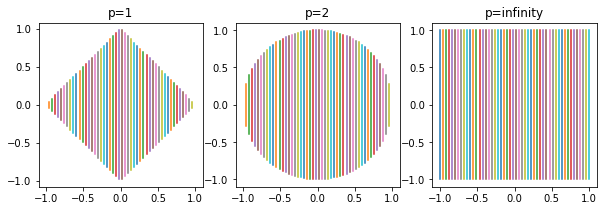
\includegraphics[width=\linewidth]{fig/pblm2_3}
	\caption{Unit Norm Ball Plots}
	\label{fig:pblm23}
\end{figure}


\begin{python}
import numpy as np
import matplotlib.plot as plt

x = np.linspace(-1,1)
y1 = 1 - abs(x)
y2 = np.sqrt(1 - x**2)
y3 = 1

fig,axs = plt.subplots(1,3,sharex=True,figsize=(10,10))

axs[0].plot([x,x],[y1,-y1])
axs[0].set_box_aspect(1)
axs[0].set_title('p=1')

axs[1].plot([x,x],[y2,-y2])
axs[1].set_box_aspect(1)
axs[1].set_title('p=2')

axs[2].plot([x,x],[y3,-y3])
axs[2].set_box_aspect(1)
axs[2].set_title('p=infinity')

\end{python}


\newpage
\subsection{Eigenvalues Proof 1}
\textbf{Problem:}
Show that the eigenvalues of $A \in \mathbf{S}^n$ are real.\\

\noindent
\textbf{Solution:}
Every eigen-value, $\lambda$, of matrix, $A \in \mathbf{S}^{n \cross n}$, must satisfy the following:
\begin{displaymath}
	A x = \lambda x, \ \forall x \in \real^n
\end{displaymath}

The following must also be true:
\begin{align*}
	x^* A x &= x^* \lambda x\\
	\qty(x^* A x)^* &= \qty(x^* \lambda x)^*\\
	x^* A^* x &= x^* \lambda^* x\\
\end{align*}

Since, by definition, $A = A^*$,
\begin{align*}
	x^* A x = x^* \lambda x &= x^* \lambda^* x = x^* A^* x\\
	\lambda &= \lambda^*
\end{align*}

This means $\lambda$ must contain no imaginary components and therefore $\lambda \in \real$.


\newpage
\subsection{Eigenvalues Proof 2}
\textbf{Problem:}
Show that for $A \in \mathbf{S}^n$,
$$A \succeq 0 \iff \lambda_i\{A\} \geq 0 ,\ \forall i = 1, \dots, n$$\\

\noindent
\textbf{Solution:}
Every eigen-value, $\lambda \in \real$, of matrix, $A \in \mathbf{S}^{n \cross n}$, must satisfy the following:
\begin{displaymath}
	A x = \lambda x, \ \forall x \in \real^n
\end{displaymath}

By definition, a semi-positive definite matrix must satisfy the following:
$$x^T A x \geq 0, \ \forall x \in \real^n$$.

The following must also be true:
\begin{align*}
	x^T A x &\geq 0\\
	x^T \qty(\lambda x) &\geq 0
	\intertext{Thus,}
	\lambda x^T x  = x^T A x &\geq 0\\
\end{align*}

Since $\lambda x^T x \geq 0 \iff \lambda \geq 0$, the following is also true:
$$A \succeq 0 \iff \lambda \geq 0$$.

\newpage
\subsection{Optimal Control Problem Derivation}
\textbf{Problem:}
Derive the solution to the finite horizon open-loop optimal control problem:
\begin{displaymath}
	\text{minimize} \ \sum_{t=0}^{N-1} \qty(\norm{z_t}_2^2 + \norm{u_t}_2^2) + \norm{z_N}_2^2
\end{displaymath}
where $z_{t+1} = A z_t + B u_t$ with given $z_0$. Take the optimization variables to be $z_t \in \real ^n$ for $t = 1,\dots,N$ and $u_t \in \real^m$ for $t = 0,\dots,N-1$.\\

\noindent
\textbf{Solution:}\\
Define the following vectors:
\begin{align*}
	\vb{z} = \mqty[z_1^T\\ \vdots \\ z_N^T] \hspace{1in} \vb{u} = \mqty[u_0^T\\ \vdots \\ u_{N-1}^T]\\
\end{align*}

$\vb{z}$ can then be redefined in terms of $\vb{u}$ and $z_0$:
\begin{align*}
\intertext{Since}
	z_{t+1} &= A z_{t} + B u_{t}\\
	z_{1} 	&= A z_{0} + B u_{0}\\
	z_{2} 	&= A z_{1} + B u_{1}\\
			&= A \qty(A z_{0} + B u_{0}) + B u{1}\\
			&= A^2 z_0 + AB u_0 + B u_1\\
	z_{3}	&= A^3 z_0 + A^2 B u_0 + A B u_1 + B u_2\\
			& \ \ \vdots\\
	z_{N}	&= A z_{N-1} + B u_{N-1}\\
			&= A^n z_0 + A^{n-1} B u_0 + \dots + A B u_{n-1} + B u_n\\
\intertext{Additonally, this can be generalized as:}
	z_{t}	&= A^{t} z_0 + \sum_{i=0}^{t-1} A^{t-i} B \vb{u}_{i}\\
\intertext{The entire sum can be vectorized as follows:}
	\vb{z}	&= \mqty[\mqty{A \\ A^2 \\ \vdots \\ A^N} 
					& \mqty{|\\|\\|\\|} 
					& \mqty{B 	& 0 & \dots & 0\\
							AB 	& B & \dots & 0\\
							\vdots & \ddots &\ddots &\vdots\\
							A^{n-1}B &\dots &AB &B}] \mqty[z_0\\ \_\_ \\ \vb{u}]\\
			&= [A_{m} | B_{m}] \mqty[z_0\\ \_\_ \\ \vb{u}]\\
			&= A_m z_0 + B_m \vb{u} \\
			&= A_p \vb{u}_p
\end{align*}


This can then be substituted into the minimization funtion:
\begin{align*}
	\sum_{t=0}^{N-1} \qty(\norm{z_t}_2^2 + \norm{u_t}_2^2) + \norm{z_N}_2^2
	&= \sum_{t=0}^{N-1} \qty(\norm{\qty(A_{p,t} \vb{u}_{p,t})^2}_2)^2 + \norm{u_t}_2^2) + \sum_{t=0}^{N-1} \frac{1}{N} \norm{z_N}_2^2\\
	&= \sum_{t=0}^{N-1} \qty( \qty(\sqrt{\sum_{i=1}^{n} \qty(A_{p,t} \vb{u}_{p,t})})^2 + \qty(\sqrt{\sum_{i=1}^{n} u_{i}^2})^2 + \frac{1}{N} \qty(\sqrt{\sum_{i=1}^{n} z_{N,i}^2})^2)\\
	&= \sum_{t=0}^{N-1} \qty(\sum_{i=1}^{n} \qty(A_{p,t} \vb{u}_{p,t})^2 + \sum_{i=1}^{n} u_{i}^2  + \frac{1}{N} \sum_{i=1}^{n} z_{N,i}^2)\\
	&= \sum_{t=0}^{N-1} \sum_{i=1}^{n} \qty( \qty(A_{p,t} \vb{u}_{p,t})^2 + u_{i}^2 + \frac{1}{N} z_{N,i}^2)\\
	&= \sum_{t=0}^{N-1} \sum_{i=1}^{n} \qty( \qty(A_{p,t} \vb{u}_{p,t})^2 + u_{i}^2 + \frac{1}{N} z_{N,i}^2)\\
\intertext{From the definition of the 2-norm for vectors and the F- norm for matrices, the following can be found:}
	&= \norm{A_p\vb{u}_p + \vb{u} + \frac{1}{N} z_N}_F^2\\
\intertext{This can then be expanded into the follwoing matrix equivelent:}
	&= \norm{A_m z_0 + B_m\vb{u} + \vb{u} + \frac{1}{N} z_N}_F^2\\
	&= \norm{A_m z_0 + \qty(B_m + I) \vb{u} + \frac{1}{N} z_N }_F^2
\end{align*}

Returning to the matrix definitions
\begin{align*}
	A_m z_0 + \qty(B_m + I) \vb{u} + \frac{1}{N} z_N
	&= \mqty[\mqty{A \\ A^2 \\ \vdots \\ A^N} 
			& \mqty{|\\|\\|\\|} 
			& \mqty{B 	& 0 & \dots & 0\\
				AB 	& B & \dots & 0\\
				\vdots & \ddots &\ddots &\vdots\\
				A^{n-1}B &\dots &AB &B}]
		\mqty[z_0\\ \_\_ \\ \vb{u}] + \vb{u} + \frac{1}{N} z_N\\
	&= A_m z_0 + B_m \vb{u} + \vb{u} + \frac{1}{N} z_N\\
	&= A_m z_0 + \qty(B_m + I) \vb{u} + \frac{1}{N} z_N
\end{align*}




The minimization function can then be written as:
\begin{align*}
	\text{minimize} \ \norm{A_m z_0 + \qty(B_m + I) \vb{u} + \frac{1}{N} z_N I}_F^2
\end{align*}

which can be achieved by setting the gradient to be zero and finding the minimum solution:

\begin{align*}
	0
	&= \grad{\norm{A_m z_0 + \qty(B_m + I) \vb{u} + \frac{z_N}{N}  I}_F^2}\\
	&= \grad{\qty(\sqrt{(A_m z_0)^T(A_m z_0) + \qty(\qty(B_m + I) \vb{u})^T \qty(\qty(B_m + I) \vb{u}) + \qty(\frac{z_N}{N})^2 I})^2}\\
	&= \grad{\qty(z_0^T A_m^T A_m z_0 + \vb{u}^T\qty(B_m + I)^T\qty(B_m + I) \vb{u} + \frac{z_N^2}{N^2} I)}\\
	&= 2 (B_m + I) \vb{u}\\
	\vb{u} &= 0
\end{align*}

This result states that the result that minimizes the objective function, since $Z_n$ doesn't have an objective value, is to have $u = 0 \ \forall t \geq 0$.

Another verification can be done alternatively by defining the new vector, $$\vb{x} = \mqty[z_0\\ --\\z_N\\ --\\ \vb{u}],$$ and similarly minimizing:

\begin{align*}
		A_x \vb{x}
		&= \mqty[\mqty{A \\ A^2 \\ \vdots \\ A^N} 
				& \mqty{|\\|\\|\\|} 
				& \mqty{\frac{1}{N} \\ \frac{1}{N} \\ \vdots \\ \frac{1}{N}}
				& \mqty{|\\|\\|\\|}
				& \mqty{B + 1 	& 0 & \dots & 0\\
						AB 	& B + 1 & \dots & 0\\
						\vdots & \ddots &\ddots &\vdots\\
						A^{n-1}B &\dots &AB &B + 1}]
			\mqty[z_0\\ --\\z_N\\ --\\ \vb{u}]\\
\end{align*}

The minimization function can then be written as:
\begin{align*}
	\text{minimize} \ \norm{A_x \vb{x}}_F^2
\end{align*}

which can be achieved by setting the gradient to be zero and finding the minimum solution:

\begin{align*}
	\grad{\norm{A_x \vb{x}}_F^2} = 0
	&= \grad{\qty(\sqrt{\vb{x}^T A_x^T A_x \vb{x}})^2}\\
	&= \grad{\ \vb{x}^T A_x^T A_x \vb{x}}\\ 
	&= 2 \vb{x} A_x\\
	&= 2 \vb{x} A_x \qty(\frac{1}{2}) A_x^{-1}\\
	\vb{x} &= 0
\end{align*}
The minimum value for this case is actually found to be the trivial case of all variables set to zero, including $z_0$ and $z_N$ if they were variables. This would indicate more restrictions are needed for a non-trivial solution.




\newpage
\bibliographystyle{unsrt}
\bibliography{mybib.bib}

\end{document}
